\documentclass[a4paper]{report}
\usepackage[utf8]{inputenc}
\usepackage[T1]{fontenc}
\usepackage{RJournal}
\usepackage{amsmath,amssymb,array}
\usepackage{booktabs}


% tightlist command for lists without linebreak
\providecommand{\tightlist}{%
  \setlength{\itemsep}{0pt}\setlength{\parskip}{0pt}}


% Always define CSL refs as bib entries are contained in separate doc
% Pandoc citation processing
\newlength{\cslhangindent}
\setlength{\cslhangindent}{1.5em}
\newlength{\csllabelwidth}
\setlength{\csllabelwidth}{3em}
\newlength{\cslentryspacingunit} % times entry-spacing
\setlength{\cslentryspacingunit}{\parskip}
% for Pandoc 2.8 to 2.10.1
\newenvironment{cslreferences}%
  {}%
  {\par}
% For Pandoc 2.11+
\newenvironment{CSLReferences}[2] % #1 hanging-ident, #2 entry spacing
 {% don't indent paragraphs
  \setlength{\parindent}{0pt}
  % turn on hanging indent if param 1 is 1
  \ifodd #1
  \let\oldpar\par
  \def\par{\hangindent=\cslhangindent\oldpar}
  \fi
  % set entry spacing
  \setlength{\parskip}{#2\cslentryspacingunit}
 }%
 {}
\usepackage{calc}
\newcommand{\CSLBlock}[1]{#1\hfill\break}
\newcommand{\CSLLeftMargin}[1]{\parbox[t]{\csllabelwidth}{#1}}
\newcommand{\CSLRightInline}[1]{\parbox[t]{\linewidth - \csllabelwidth}{#1}\break}
\newcommand{\CSLIndent}[1]{\hspace{\cslhangindent}#1}



\begin{document}


%% do not edit, for illustration only
\sectionhead{Contributed research article}
\volume{14}
\volnumber{4}
\year{2022}
\month{December}
\setcounter{page}{305}

\begin{article}
  % !TeX root = RJwrapper.tex
\title{TreeSearch: Morphological Phylogenetic Analysis in R}
\author{by Martin R. Smith}

\maketitle

\abstract{%
\CRANpkg{TreeSearch} is an R package for phylogenetic analysis, optimized for discrete character data. Tree search may be conducted using equal or implied step weights with an explicit (albeit inexact) allowance for inapplicable character entries, avoiding some of the pitfalls inherent in standard parsimony methods. Profile parsimony and user-specified optimality criteria are supported.
A graphical interface, which requires no familiarity with R, is designed to help a user to improve the quality of datasets through critical review of underpinning character codings; and to obtain additional information from results by identifying and summarizing clusters of similar trees, mapping the distribution of trees, and removing `rogue' taxa that obscure underlying relationships.
Taken together, the package aims to support methodological rigour at each step of data collection, analysis, and the exploration of phylogenetic results.
}

\hypertarget{introduction}{%
\section{Introduction}\label{introduction}}

Even in the phylogenomic era, morphological data make an important contribution
to phylogenetic questions. Discrete phenotypic data improve the accuracy and
resolution of phylogenetic reconstruction even when outnumbered by molecular
characters, and are the only way to incorporate the unique perspective on
historical events that fossil taxa provide (Wiens 2004; Wortley and Scotland 2006; Koch and Parry 2020; Asher and Smith 2022).

One challenge with morphological analysis is the treatment of inapplicable
character states: for example, `tail colour' cannot logically be ascribed either
of the states `red' or `blue' in a taxon that lacks a tail (W. P. Maddison 1993). This
situation can profoundly mislead phylogenetic analysis, and is not handled
appropriately by any standard Markov model or parsimony method.

Solutions to this issue have recently been proposed (De Laet 2005; Brazeau, Guillerme, and Smith 2019; Tarasov 2019, 2022; Goloboff et al. 2021; Hopkins and St. John 2021). Where a single
`principal' character (e.g.~`tail') exhibits \(n\) `contingent' characters (e.g.
`tail colour', `tail covering'), `exact' solutions (Tarasov 2019, 2022; Goloboff et al. 2021) require the construction of multi-state hierarchies containing
\(O(2^n)\) entries, meaning that analysis is only computationally tractable for
simple hierarchies with few contingent characters. Moreover, these approaches
cannot accommodate characters that are contingent on more than one principal
character: for example, characters describing appendages on a differentiated
head may be contingent on the presence of the two characters `appendages' and
`differentiated head'.

Such situations can be approached using the flexible parsimony approximation
proposed by Brazeau, Guillerme, and Smith (2019). \pkg{TreeSearch} scores trees using the ``Morphy'' C
implementation of this algorithm (Brazeau, Smith, and Guillerme 2017). Morphy implements tree search
under equal step weights. TreeSearch additionally implements implied step
weighting (Goloboff 1993), a method which consistently finds more accurate and
precise trees than equal weights parsimony (Goloboff et al. 2008; Goloboff, Torres, and Arias 2018; M. R. Smith 2019a).

There has been lively discussion as to whether, with the rise of probabilistic
approaches, parsimony remains a useful tool for morphological phylogenetics
(e.g. O'Reilly et al. 2016; Puttick et al. 2017; Sansom et al. 2018; Goloboff, Torres Galvis, and Arias 2018; Brown et al. 2017).
Notwithstanding scenarios that go beyond the limits of parsimony, such as the
simultaneous incorporation of stratigraphic data and other prior knowledge (e.g. Guenser et al. 2021), neither parsimony nor probabilistic methods consistently recover
`better' trees when gains in accuracy are balanced against losses in precision
(M. R. Smith 2019a). Even if probabilistic methods may eventually be improved through
the creation of more sophisticated models that better reflect the nature of
morphological data (Goloboff, Torres, and Arias 2018; Tarasov 2019, 2022), parsimony
analysis remains a useful tool -- not only because treatments of inapplicable
character states are presently available, but also because it facilitates a
deeper understanding of the underpinning data by emphasizing the reciprocal
relationship between a tree and the synapomorphies that it implies.

Whatever method is used to find phylogenetic trees, a single consensus tree may
fail to convey all the signal in a set of phylogenetic results (Wilkinson 1994, 1996, 2003). A set of optimal trees can be better
interpreted by examining consensus trees generated from clusters of similar
trees (Stockham, Wang, and Warnow 2002); by exploring tree space (Wright and Lloyd 2020; M. R. Smith 2022a) and by
automatically identifying, annotating and removing `wildcard' taxa (M. R. Smith 2022b)
whose `rogue' behaviour may reflect underlying character conflict or ambiguity
(Kearney 2002). These methods are not always easy to integrate into phylogenetic
workflows, so are not routinely included in empirical studies.

\begin{figure}

{\centering 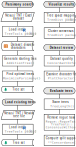
\includegraphics[width=0.6\linewidth]{Flow} 

}

\caption{Flow charts summarizing key functions available in TreeSearch.}\label{fig:flowchart}
\end{figure}

TreeSearch provides functions that allow researchers to engage with the three
main aspects of morphological phylogenetic analysis: dataset construction and
validation; phylogenetic search (including with inapplicable data); and the
interrogation of optimal tree sets (Fig. \ref{fig:flowchart}). These functions
can be accessed via the R command-line, as documented within the package and at
\href{https://ms609.github.io/TreeSearch/}{ms609.github.io/TreeSearch}, or through a
graphical user interface (GUI). The GUI includes options to export a log of
executed commands as a fully reproducible R script, and to save outputs in
graphical, Nexus or Newick formats.

\hypertarget{implementation}{%
\section{Implementation}\label{implementation}}

\hypertarget{tree-scoring}{%
\subsection{Tree scoring}\label{tree-scoring}}

\pkg{TreeSearch} can score trees using equal weights, implied weighting
(Goloboff 1993), or profile parsimony (Faith and Trueman 2001). The function \texttt{TreeLength()}
calculates tree score using the ``Morphy'' phylogenetic library (Brazeau, Smith, and Guillerme 2017),
which implements the Fitch (1971) and Brazeau, Guillerme, and Smith (2019) algorithms. Morphy returns the
equal weights parsimony score of a tree against a given dataset. Implied weights
and profile parsimony scores are computed by first making a separate call to
Morphy for each character in turn, passed as a single-character dataset; then
passing this value to the appropriate weighting formula and summing the total
score over all characters.

Implied weighting (Goloboff 1993) is an approximate method that treats each
additional step (i.e.~transition between tokens) in a character as less
surprising -- and thus requiring less penalty -- than the previous step. Each
additional step demonstrates that a character is less reliable for phylogenetic
inference, and thus more likely to contain additional homoplasy. The score of a
tree under implied weighting is \(\sum{\frac{e_i}{e_i+k}}\), where \(e_i\) denotes
the number of extra steps observed in character \(i\), and is derived by
subtracting the minimum score that the character can obtain on any tree from the
score observed on the tree in question (Goloboff 1993). The minimum length of a
tree is one less than the number of unique tokens (excluding the inapplicable
token `\texttt{-}') that must be present.

Profile parsimony (Faith and Trueman 2001) represents an alternative formulation of how
surprising each additional step in a character is (Arias and Miranda-Esquivel 2004): the penalty
associated with each additional step in a character is a function of the
probability that a character will fit at least as well as is observed on a
uniformly selected tree. On this view, an additional step is less surprising if
observed in a character where there are more opportunities to observe homoplasy,
whether because a character contains fewer ambiguous codings (a motivation for
the `extended' implied weighting of Goloboff (2014)) or because states are
distributed more evenly in a character, whose higher phylogenetic information
content (Thorley, Wilkinson, and Charleston 1998) corresponds to a lower proportion of trees in which no
additional steps are observed.

TreeSearch calculates the profile parsimony score by computing the logarithm of
the number of trees onto which a character can be mapped using \(m\) steps, using
theorem 1 of Carter et al. (1990). As computation for higher numbers of states
(W. P. Maddison and Slatkin 1991) is more computationally complex, the present implementation is
restricted to characters that contain two informative applicable states, and
uses the Fitch (1971) algorithm.

\hypertarget{tree-search}{%
\subsection{Tree search}\label{tree-search}}

The TreeSearch GUI uses the routine \texttt{MaximizeParsimony()} to search for optimal
trees using tree bisection and reconnection (TBR) searches and the parsimony
ratchet (Nixon 1999). This goes beyond the heuristic tree search implementation
in the R package \CRANpkg{phangorn} (Schliep 2011) by using compiled C++ code to
rearrange trees, dramatically accelerating computation, and thus increasing the
scale of dataset that can be analysed in reasonable time; and in supporting TBR
rearrangements, which explore larger neighbourhoods of tree space: TBR evaluates
more trees than nearest-neighbour interchanges or subtree pruning and
regrafting, leading to additional computational expense that is offset by a
decreased likelihood that search will become trapped in a local optimum
(Goeffon, Richer, and Jin-Kao Hao 2008; Whelan and Money 2010).

By default, search begins from a greedy addition tree generated by function
\texttt{AdditionTree()}, which queues taxa in a random order, then attaches each taxon
in turn to the growing tree at the most parsimonious location. Search may also
be started from neighbour-joining trees, or the results of a previous search.

Search commences by conducting TBR rearrangements -- a hill-climbing approach
that locates a locally optimal tree from which no tree accessible by a single
TBR rearrangement has a better score. A TBR iteration breaks a randomly selected
edge in the focal tree, and reconnects each possible pair of edges in the
resultant sub-trees to produce a list of candidate trees. Entries that are
inconsistent with user-specified topological constraints are removed; remaining
trees are inserted into a queue and scored in a random sequence. If the score of
a candidate tree is at least as good as the best yet encountered (within the
bounds of an optional tolerance parameter \(\epsilon\), which allows the retention
of almost-optimal trees in order to improve accuracy -- see e.g. M. R. Smith (2019a)),
this tree is used as the starting point for a new TBR iteration. Otherwise, the
next tree in the list is considered. TBR search continues until the best score
is found a specified number of times; a specified number of TBR break points
have been evaluated without any improvement to tree score; or a set amount of
time has passed.

When TBR search is complete, iterations of the parsimony ratchet (Nixon 1999)
are conducted in order to search areas of tree space that are separated from the
best tree yet found by `valleys' that cannot be traversed by TBR rearrangements
without passing through trees whose optimality score is below the threshold for
acceptance. Each ratchet iteration begins by resampling the original matrix. A
round of TBR search is conducted using this resampled matrix, and the tree thus
produced is used as a starting point for a new round of TBR search using the
original data. After a specified number of ratchet iterations, an optional final
round of TBR search allows a denser sampling of optimal trees from the final
region of tree space.

A simple example search can be conducted using a morphological dataset included
in the package, taken from Vinther, Van Roy, and Briggs (2008):

\begin{verbatim}
library("TreeSearch")
vinther <- inapplicable.phyData[["Vinther2008"]]
trees <- MaximizeParsimony(vinther, concavity = 10, tolerance = 0.05)
\end{verbatim}

The \texttt{MaximizeParsimony()} command performs tree search under implied weights
with a concavity value of 10 (\texttt{concavity\ =\ Inf} would select equal weights),
retaining any tree whose score is within 0.05 of the best score.

The resulting trees can be summarised according to their scores (optionally,
against a different \texttt{dataset} or under a different weighting strategy, as
specified by \texttt{concavity}) and the iteration in which they were first hit:

\begin{verbatim}
TreeLength(trees, dataset = vinther, concavity = 10) |> 
  signif() |>         # truncate non-significant digits
  table()             # tabulate by score
\end{verbatim}

\begin{verbatim}
#> 
#> 1.52814 1.54329  1.5641 
#>       3      45       4
\end{verbatim}

\begin{verbatim}
attr(trees, "firstHit")
\end{verbatim}

\begin{verbatim}
#>   seed  start ratch1 ratch2 ratch3 ratch4 ratch5 ratch6 ratch7  final 
#>      0     29      4      0     10      7      2      0      0      0
\end{verbatim}

More flexible, if less computationally efficient, tree searches can be conducted
at the command line using the \texttt{TreeSearch()}, \texttt{Ratchet()} and \texttt{Bootstrap()}
commands, which support custom tree optimality criteria (e.g. Hopkins and St. John 2021).

\hypertarget{visualization}{%
\subsection{Visualization}\label{visualization}}

The distribution of optimal trees, however obtained, can be visualized through
interactive mappings of tree space (Hillis, Heath, and St. John 2005; M. R. Smith 2022a). The TreeSearch GUI supports the use of information theoretic distances
(M. R. Smith 2020a); the quartet distance (Estabrook, McMorris, and Meacham 1985); or the Robinson--Foulds
distance (Robinson and Foulds 1981) to construct tree spaces, which are mapped into 2--12
dimensions using principal coordinates analysis (Gower 1966). The degree to
which a mapping faithfully depicts original tree-to-tree distances is measured
using the product of the trustworthiness and continuity metrics (Venna and Kaski 2001; Kaski et al. 2003; M. R. Smith 2022a), a composite score denoting the degree to which points
that are nearby when mapped are truly close neighbours (trustworthiness), and
the degree to which nearby points remain nearby when mapped (continuity).
Plotting the minimum spanning tree -- the shortest path that connects all trees
(Gower and Ross 1969) -- can highlight stress in a mapping (grey lines in Fig.
\ref{fig:treespace-latex}): the spatial relationships of trees are distorted in
regions where the minimum spanning tree takes a circuitous route to connect
trees that are mapped close to one another (see fig.~1a--b in M. R. Smith 2022a).

\begin{figure}
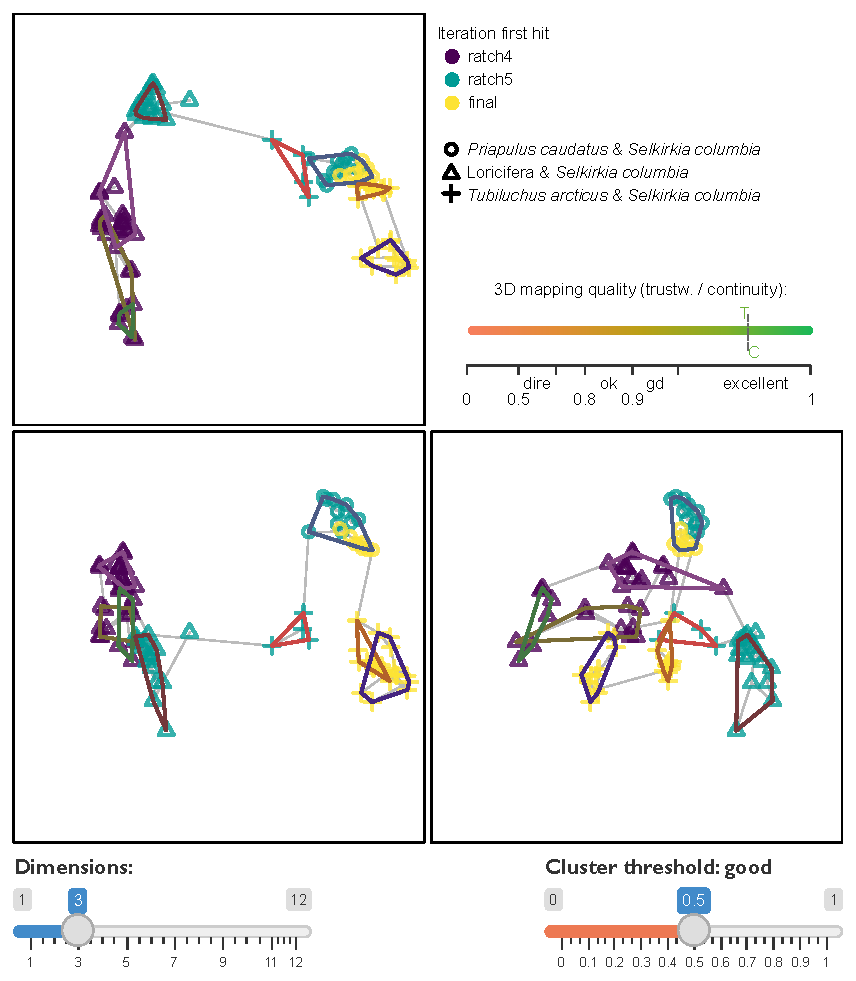
\includegraphics[width=1\linewidth]{TreeSpace} \caption{Three-dimensional map visualizing progress in a tree search in the TreeSearch GUI. Optimal trees belong to three statistically distinct clusters with good support (silhouette coefficient \(>\) 0.5), characterized by different relationships between certain taxa (plotting symbols). Although multiple ratchet iterations have visited each cluster, limited overlap between ratchet iterations suggests that a continuation of tree search may sample novel optimal trees. High trustworthiness and continuity values and a simple minimum spanning tree (grey) indicate that the mapping does not exhibit severe distortion. This figure depicts the tree space GUI display after loading the Wills et al. (2012) dataset; clearing previous trees from memory (sample \emph{n} trees = 0); and starting a new search (Search→Configure) with equal step weighting and \(10^{1.5}\) max hits. 93 trees were sampled, coloured by ``When first found'', with plotting symbols depicting ``Relationships'' between the specified taxa.}\label{fig:treespace-latex}
\end{figure}



To relate the geometry of tree space to the underlying trees, each point in tree
space may be annotated according to the optimality score of its corresponding
tree under a selected step weighting scheme; by the relationships between chosen
taxa that are inferred by that tree; and by the search iteration in which the
tree was first found by tree search (Fig. \ref{fig:treespace-latex}).

Annotating trees by the iteration in which they were first found allows a user
to evaluate whether a continuation of tree search is likely to yield more
optimal trees. For example, if the retained trees were only recently found, the
search may not yet have located a global optimum. Alternatively, if certain
regions of tree space are visited only by a single ratchet iteration, it is
possible that further isolated `islands' (Bastert et al. 2002) remain to be found;
continuing tree search until subsequent ratchet iterations no longer locate new
clusters of trees will reduce the chance that optimal regions of tree space
remain unvisited.

As the identification of clusters from mappings of tree space can be misleading
(M. R. Smith 2022a), TreeSearch identifies clusters of trees from tree-to-tree
distances using K-means++ clustering, partitioning around medoids and
hierarchical clustering with minimax linkage (Hartigan and Wong 1979; Arthur and Vassilvitskii 2007; Murtagh 1983; Bien and Tibshirani 2011; Maechler et al. 2019). Clusterings are evaluated using the
silhouette coefficient, a measure of the extent of overlap between clusters
(Kaufman and Rousseeuw 1990). The clustering with the highest silhouette coefficient is
depicted if the silhouette coefficient exceeds a user-specified threshold; the
interpretation of the chosen threshold according to Kaufman and Rousseeuw (1990) is displayed to
the user. Plotting a separate consensus tree for each cluster often reveals
phylogenetic information that is concealed by polytomies in the single `plenary'
consensus of all optimal trees (Stockham, Wang, and Warnow 2002).

Plenary consensus trees can also lack resolution because of wildcard or `rogue'
taxa, in which conflict or ambiguity in their character codings leads to an
unsettled phylogenetic position (Wilkinson 1994, 2003; Kearney 2002).
TreeSearch detects rogue taxa using a heuristic approach (M. R. Smith 2022b) that
seeks to maximize the phylogenetic information content (\emph{sensu} Thorley, Wilkinson, and Charleston 1998) of
a consensus tree created after removing rogue taxa from input trees. The
position of an excluded taxon is portrayed by shading each edge or node of the
consensus according to the number of times the specified taxon occurs at that
position on an underlying tree
{[}Fig. \ref{fig:rogueplot-latex}; after
Klopfstein and Spasojevic (2019){]}, equivalent to the `branch attachment frequency' of Phyutility
(S. A. Smith and Dunn 2008).

Identifying taxa with an unstable position, and splits with low support, can
help an investigator to critically re-examine character codings; to this end,
each edge of the resulting consensus can be annotated with the frequency of the
split amongst the tree set, or with a concordance factor (Minh, Hahn, and Lanfear 2020) denoting
the strength of support from the underlying dataset.

\begin{figure}
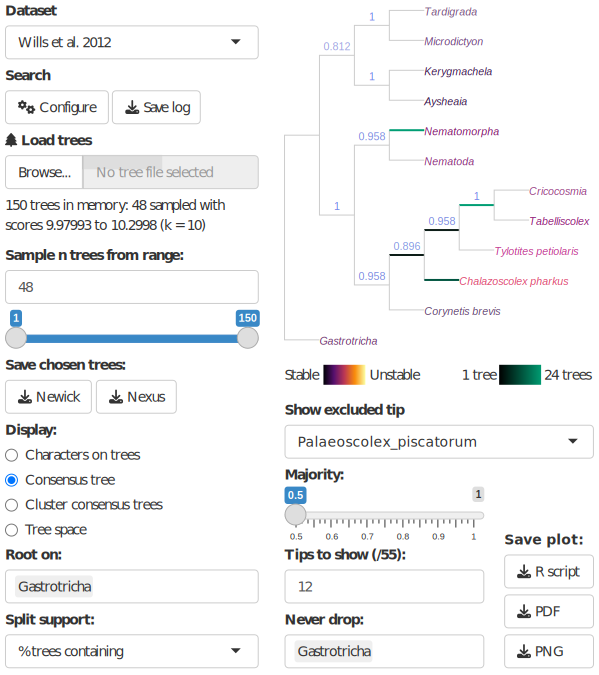
\includegraphics[width=1\linewidth]{WillsCons} \caption{Reduced consensus of 48 cladograms generated by analysis of data from Wills et al. (2012) under different parsimony methods by Brazeau, Guillerme, and Smith (2019), as displayed in the TreeSearch graphical user interface. Removal of taxa reveals strong support for relationships that would otherwise be masked by rogues such as \emph{Palaeoscolex}, whose position in optimal trees is marked by the highlighted edges. The GUI state can be reproduced by selecting the options displayed in the figure.}\label{fig:rogueplot-latex}
\end{figure}



\hypertarget{dataset-review}{%
\subsection{Dataset review}\label{dataset-review}}

Ultimately, the quality of a dataset plays a central role in determining the
reliability of phylogenetic results, with changes to a relatively small number
of character codings potentially exhibiting an outsized impact on reconstructed
topologies (Goloboff and Sereno 2021). Nevertheless, dataset quality does not always
receive commensurate attention (Simões et al. 2017). One step towards improving the
rigour of morphological datasets is to annotate each cell in a dataset with an
explicit justification for each taxon's coding (Sereno 2009), which can be
accomplished in Nexus-formatted data files (D. R. Maddison, Swofford, and Maddison 1997) using software such
as \href{https://morphobank.org}{MorphoBank} (O'Leary and Kaufman 2011).

TreeSearch presents such annotations alongside a reconstruction of each
character's states on a specified tree, with inapplicable states mapped
according to the algorithm of Brazeau, Guillerme, and Smith (2019). Neomorphic (presence/absence) and
transformational characters (Sereno 2007) are distinguished by reserving the
token \texttt{0} to solely denote the absence of a neomorphic character, with tokens
\texttt{1} \ldots{} \texttt{n} used to denote the \(n\) states of a transformational character
(Brazeau, Guillerme, and Smith 2019). In order to identify character codings that contribute to taxon
instability, each leaf is coloured according to its mean contribution to tree
length for the visualized character (Pol and Escapa 2009).

This visualization of reconstructed character transitions can help to identify
cases where the formulation of characters has unintended consequences
(Wilkinson 1995; Brazeau 2011); where inapplicable states have been
inconsistently applied (Brazeau, Guillerme, and Smith 2019); where taphonomic absence is wrongly coded
as biological absence (Donoghue and Purnell 2009); where previous datasets are uncritically
recycled (Jenner 2001); or where taxa are coded with more confidence than a
critical evaluation of available evidence can truly support. Insofar as the
optimal tree and the underlying characters are reciprocally illuminating
(Mooi and Gill 2016), successive cycles of phylogenetic analysis and character
re-formulation can improve the integrity of morphological datasets, and thus
increase their capacity to yield meaningful phylogenetic results (Hennig 1966).

\hypertarget{availability}{%
\section{Availability}\label{availability}}

\CRANpkg{TreeSearch} can be installed through the Comprehensive R Archive
Network (CRAN) using\break
\texttt{install.packages("TreeSearch")}; the graphical user
interface is launched with the command\break
\texttt{TreeSearch::EasyTrees()}.
The package has been tested on Windows 10, Mac OS X 10 and Ubuntu 20, and
requires only packages available from the CRAN repository.
Source code is available at \url{https://github.com/ms609/TreeSearch/},
and is permanently archived at Zenodo
(\url{https://dx.doi.org/10.5281/zenodo.1042590}). Online documentation is available
at \url{https://ms609.github.io/TreeSearch/}.

\hypertarget{acknowledgements}{%
\section{Acknowledgements}\label{acknowledgements}}

I thank Alavya Dhungana and Joe Moysiuk for feedback on preliminary versions of
the software, and Martin Brazeau and anonymous referees for comments on the
manuscript. Functionality in TreeSearch employs the underlying R
packages \CRANpkg{ape} (Paradis and Schliep 2019), \CRANpkg{phangorn} (Schliep 2011),
\CRANpkg{Quartet} (Sand et al. 2014; M. R. Smith 2019b), \CRANpkg{Rogue} (M. R. Smith 2022b),
\CRANpkg{shiny} (Chang et al. 2021), \CRANpkg{shinyjs} (Attali 2020), \CRANpkg{TreeDist}
(M. R. Smith 2020b), and \CRANpkg{TreeTools} (M. R. Smith 2019c). Icons from R used under
GPL-3; Font Awesome, CC-BY-4.0.

\hypertarget{references}{%
\section*{References}\label{references}}
\addcontentsline{toc}{section}{References}

\hypertarget{refs}{}
\begin{CSLReferences}{1}{0}
\leavevmode\vadjust pre{\hypertarget{ref-Arias2004}{}}%
Arias, J. Salvador, and Daniel Rafael Miranda-Esquivel. 2004. {``Profile Parsimony ({PP}): An Analysis Under Implied Weights ({IW}).''} \emph{Cladistics} 20 (1): 56--63. \url{https://doi.org/10.1111/j.1096-0031.2003.00001.x}.

\leavevmode\vadjust pre{\hypertarget{ref-Arthur2007}{}}%
Arthur, David, and Sergei Vassilvitskii. 2007. {``K-Means++: The Advantages of Careful Seeding.''} In \emph{Proceedings of the Eighteenth Annual {ACM-SIAM} Symposium on {Discrete} Algorithms}, 1027--35. {SODA} '07. {USA}: {Society for Industrial and Applied Mathematics}. \url{https://dl.acm.org/doi/10.5555/1283383.1283494}.

\leavevmode\vadjust pre{\hypertarget{ref-Asher2021}{}}%
Asher, Robert J., and Martin R. Smith. 2022. {``Phylogenetic Signal and Bias in Paleontology.''} \emph{Systematic Biology} 71 (4): 986--1008. \url{https://doi.org/10.1093/sysbio/syab072}.

\leavevmode\vadjust pre{\hypertarget{ref-shinyjs}{}}%
Attali, Dean. 2020. \emph{Shinyjs: Easily Improve the User Experience of Your Shiny Apps in Seconds}. \url{https://CRAN.R-project.org/package=shinyjs}.

\leavevmode\vadjust pre{\hypertarget{ref-Bastert2002}{}}%
Bastert, Oliver, Dan Rockmore, Peter F. Stadler, and Gottfried Tinhofer. 2002. {``Landscapes on Spaces of Trees.''} \emph{Applied Mathematics and Computation} 131 (2-3): 439--59. \url{https://doi.org/10.1016/S0096-3003(01)00164-3}.

\leavevmode\vadjust pre{\hypertarget{ref-Bien2011}{}}%
Bien, Jacob, and Robert Tibshirani. 2011. {``Hierarchical Clustering with Prototypes via Minimax Linkage.''} \emph{Journal of the American Statistical Association} 106 (495): 1075--84. \url{https://doi.org/10.1198/jasa.2011.tm10183}.

\leavevmode\vadjust pre{\hypertarget{ref-Brazeau2011}{}}%
Brazeau, Martin D. 2011. {``Problematic Character Coding Methods in Morphology and Their Effects.''} \emph{Biological Journal of the Linnean Society} 104 (3): 489--98. \url{https://doi.org/10.1111/j.1095-8312.2011.01755.x}.

\leavevmode\vadjust pre{\hypertarget{ref-Brazeau2019}{}}%
Brazeau, Martin D., Thomas Guillerme, and Martin R. Smith. 2019. {``An Algorithm for Morphological Phylogenetic Analysis with Inapplicable Data.''} \emph{Systematic Biology} 68 (4): 619--31. \url{https://doi.org/10.1093/sysbio/syy083}.

\leavevmode\vadjust pre{\hypertarget{ref-Brazeau2017}{}}%
Brazeau, Martin D., Martin R. Smith, and Thomas Guillerme. 2017. {``{MorphyLib}: A Library for Phylogenetic Analysis of Categorical Trait Data with Inapplicability.''} \url{https://doi.org/10.5281/zenodo.815372}.

\leavevmode\vadjust pre{\hypertarget{ref-Brown2017}{}}%
Brown, Joseph W., Caroline Parins-Fukuchi, Gregory W. Stull, Oscar M. Vargas, and Stephen A. Smith. 2017. {``Bayesian and Likelihood Phylogenetic Reconstructions of Morphological Traits Are Not Discordant When Taking Uncertainty into Consideration: A Comment on {Puttick} {\emph{Et Al.}}''} \emph{Proceedings of the Royal Society B: Biological Sciences} 284 (1864): 20170986. \url{https://doi.org/10.1098/rspb.2017.0986}.

\leavevmode\vadjust pre{\hypertarget{ref-Carter1990}{}}%
Carter, M., M. Hendy, D. Penny, L. A. Székely, and N. C. Wormald. 1990. {``On the Distribution of Lengths of Evolutionary Trees.''} \emph{SIAM Journal on Discrete Mathematics} 3 (1): 38--47. \url{https://doi.org/10.1137/0403005}.

\leavevmode\vadjust pre{\hypertarget{ref-shiny}{}}%
Chang, Winston, Joe Cheng, J. J. Allaire, Carson Sievert, Barret Schloerke, Yi-Hui Xie, Jeff Allen, Jonathan McPherson, Alan Dipert, and Barbara Borges. 2021. \emph{Shiny: Web Application Framework for {R}}. \url{https://CRAN.R-project.org/package=shiny}.

\leavevmode\vadjust pre{\hypertarget{ref-DeLaet2005}{}}%
De Laet, Jan E. 2005. {``Parsimony and the Problem of Inapplicables in Sequence Data.''} Edited by V. A. Albert. \emph{Parsimony, Phylogeny, and Genomics}, 81--116. \url{https://doi.org/10.1093/acprof:oso/9780199297306.003.0006}.

\leavevmode\vadjust pre{\hypertarget{ref-Donoghue2009}{}}%
Donoghue, Philip C. J., and Mark A. Purnell. 2009. {``Distinguishing Heat from Light in Debate over Controversial Fossils.''} \emph{BioEssays} 31 (2): 178--89. \url{https://doi.org/10.1002/bies.200800128}.

\leavevmode\vadjust pre{\hypertarget{ref-Estabrook1985}{}}%
Estabrook, George F., F. R. McMorris, and Christopher A. Meacham. 1985. {``Comparison of Undirected Phylogenetic Trees Based on Subtrees of Four Evolutionary Units.''} \emph{Systematic Zoology} 34 (2): 193--200. \url{https://doi.org/10.2307/sysbio/34.2.193}.

\leavevmode\vadjust pre{\hypertarget{ref-Faith2001}{}}%
Faith, Daniel P., and John W. H. Trueman. 2001. {``Towards an Inclusive Philosophy for Phylogenetic Inference.''} \emph{Systematic Biology} 50 (3): 331--50. \url{https://doi.org/10.1080/10635150118627}.

\leavevmode\vadjust pre{\hypertarget{ref-Fitch1971}{}}%
Fitch, Walter M. 1971. {``Toward Defining the Course of Evolution: Minimum Change for a Specific Tree Topology.''} \emph{Systematic Biology} 20 (4): 406--16. \url{https://doi.org/10.1093/sysbio/20.4.406}.

\leavevmode\vadjust pre{\hypertarget{ref-Goeffon2008}{}}%
Goeffon, A., J.-M. Richer, and Jin-Kao Hao. 2008. {``Progressive {Tree Neighborhood} Applied to the {Maximum Parsimony} Problem.''} \emph{IEEE/ACM Transactions on Computational Biology and Bioinformatics} 5 (1): 136--45. \url{https://doi.org/10.1109/TCBB.2007.1065}.

\leavevmode\vadjust pre{\hypertarget{ref-Goloboff1993}{}}%
Goloboff, Pablo A. 1993. {``Estimating Character Weights During Tree Search.''} \emph{Cladistics} 9 (1): 83--91. \url{https://doi.org/10.1111/j.1096-0031.1993.tb00209.x}.

\leavevmode\vadjust pre{\hypertarget{ref-Goloboff2014}{}}%
---------. 2014. {``Extended Implied Weighting.''} \emph{Cladistics} 30 (3): 260--72. \url{https://doi.org/10.1111/cla.12047}.

\leavevmode\vadjust pre{\hypertarget{ref-Goloboff2008}{}}%
Goloboff, Pablo A., James M. Carpenter, J. Salvador Arias, and Daniel Rafael Miranda Esquivel. 2008. {``Weighting Against Homoplasy Improves Phylogenetic Analysis of Morphological Data Sets.''} \emph{Cladistics} 24 (5): 758--73. \url{https://doi.org/10.1111/j.1096-0031.2008.00209.x}.

\leavevmode\vadjust pre{\hypertarget{ref-Goloboff2021}{}}%
Goloboff, Pablo A., Jan De Laet, Duniesky Ríos-Tamayo, and Claudia A. Szumik. 2021. {``A Reconsideration of Inapplicable Characters, and an Approximation with Step-Matrix Recoding.''} \emph{Cladistics} 37 (5): 596--629. \url{https://doi.org/10.1111/cla.12456}.

\leavevmode\vadjust pre{\hypertarget{ref-Goloboff2021a}{}}%
Goloboff, Pablo A., and Paul C. Sereno. 2021. {``Comparative Cladistics: Identifying the Sources for Differing Phylogenetic Results Between Competing Morphology-Based Datasets.''} \emph{Journal of Systematic Palaeontology}, 1--26. \url{https://doi.org/10.1080/14772019.2021.1970038}.

\leavevmode\vadjust pre{\hypertarget{ref-Goloboff2018}{}}%
Goloboff, Pablo A., Ambrosio Torres, and J. Salvador Arias. 2018. {``Weighted Parsimony Outperforms Other Methods of Phylogenetic Inference Under Models Appropriate for Morphology.''} \emph{Cladistics} 34 (4): 407--37. \url{https://doi.org/10.1111/cla.12205}.

\leavevmode\vadjust pre{\hypertarget{ref-Goloboff2018b}{}}%
Goloboff, Pablo A., Ambrosio Torres Galvis, and J. Salvatdor Arias. 2018. {``Parsimony and Model-Based Phylogenetic Methods for Morphological Data: Comments on {O}'{Reilly} \emph{Et Al}.''} \emph{Palaeontology} 61 (4): 625--30. \url{https://doi.org/10.1111/pala.12353}.

\leavevmode\vadjust pre{\hypertarget{ref-Gower1966}{}}%
Gower, J. C. 1966. {``Some Distance Properties of Latent Root and Vector Methods Used in Multivariate Analysis.''} \emph{Biometrika} 53 (3/4): 325--38. \url{https://doi.org/10.2307/2333639}.

\leavevmode\vadjust pre{\hypertarget{ref-Gower1969}{}}%
Gower, J. C., and G. J. S. Ross. 1969. {``Minimum Spanning Trees and Single Linkage Cluster Analysis.''} \emph{Journal of the Royal Statistical Society. Series C (Applied Statistics)} 18 (1): 54--64. \url{https://doi.org/10.2307/2346439}.

\leavevmode\vadjust pre{\hypertarget{ref-Guenser2021}{}}%
Guenser, Pauline, Rachel C. M. Warnock, Walker Pett, Philip C. J. Donoghue, and Emilia Jarochowska. 2021. {``Does Time Matter in Phylogeny? A Perspective from the Fossil Record.''} \emph{bioR{\(\chi\)}iv}. \url{https://doi.org/10.1101/2021.06.11.445746}.

\leavevmode\vadjust pre{\hypertarget{ref-Hartigan1979}{}}%
Hartigan, J. A., and M. A. Wong. 1979. {``Algorithm {AS} 136: A {\emph{K}}-Means Clustering Algorithm.''} \emph{Journal of the Royal Statistical Society. Series C (Applied Statistics)} 28 (1): 100--108. \url{https://doi.org/10.2307/2346830}.

\leavevmode\vadjust pre{\hypertarget{ref-Hennig1966}{}}%
Hennig, Willi. 1966. \emph{Phylogenetic Systematics}. {Urbana}: {The University of Illinois Press}.

\leavevmode\vadjust pre{\hypertarget{ref-Hillis2005}{}}%
Hillis, David M., Tracy A. Heath, and Katherine St. John. 2005. {``Analysis and Visualization of Tree Space.''} \emph{Systematic Biology} 54 (3): 471--82. \url{https://doi.org/10.1080/10635150590946961}.

\leavevmode\vadjust pre{\hypertarget{ref-Hopkins2021}{}}%
Hopkins, Melanie J., and Katherine St. John. 2021. {``Incorporating Hierarchical Characters into Phylogenetic Analysis.''} \emph{Systematic Biology} 70 (6): 1163--80. \url{https://doi.org/10.1093/sysbio/syab005}.

\leavevmode\vadjust pre{\hypertarget{ref-Jenner2001}{}}%
Jenner, Ronald A. 2001. {``Bilaterian Phylogeny and Uncritical Recycling of Morphological Data Sets.''} Edited by R. Olmstead. \emph{Systematic Biology} 50 (5): 730--42. \url{https://doi.org/10.1080/106351501753328857}.

\leavevmode\vadjust pre{\hypertarget{ref-Kaski2003}{}}%
Kaski, Samuel, Janne Nikkilä, Merja Oja, Jarkko Venna, Petri Törönen, and Eero Castrén. 2003. {``Trustworthiness and Metrics in Visualizing Similarity of Gene Expression.''} \emph{BMC Bioinformatics} 4: 48. \url{https://doi.org/10.1186/1471-2105-4-48}.

\leavevmode\vadjust pre{\hypertarget{ref-Kaufman1990}{}}%
Kaufman, Leonard, and Peter J. Rousseeuw. 1990. {``Partitioning Around Medoids ({Program PAM}).''} In \emph{Finding Groups in Data: An Introduction to Cluster Analysis}, 68--125. Wiley {Series} in {Probability} and {Statistics}. {John Wiley \& Sons, Ltd}.

\leavevmode\vadjust pre{\hypertarget{ref-Kearney2002}{}}%
Kearney, Maureen. 2002. {``Fragmentary Taxa, Missing Data, and Ambiguity: Mistaken Assumptions and Conclusions.''} \emph{Systematic Biology} 51 (2): 369--81. \url{https://doi.org/10.1080/10635150252899824}.

\leavevmode\vadjust pre{\hypertarget{ref-Klopfstein2019}{}}%
Klopfstein, Seraina, and Tamara Spasojevic. 2019. {``Illustrating Phylogenetic Placement of Fossils Using {RoguePlots}: An Example from Ichneumonid Parasitoid Wasps ({Hymenoptera}, {Ichneumonidae}) and an Extensive Morphological Matrix.''} \emph{PLoS ONE} 14 (4): e0212942. \url{https://doi.org/10.1371/journal.pone.0212942}.

\leavevmode\vadjust pre{\hypertarget{ref-Koch2020}{}}%
Koch, Nicolás Mongiardino, and Luke A. Parry. 2020. {``Death Is on Our Side: Paleontological Data Drastically Modify Phylogenetic Hypotheses.''} \emph{Systematic Biology} 69 (6): 1052--67. \url{https://doi.org/10.1093/sysbio/syaa023}.

\leavevmode\vadjust pre{\hypertarget{ref-Maddison1997}{}}%
Maddison, David R., David L. Swofford, and Wayne P. Maddison. 1997. {``{NEXUS}: An Extensible File Format for Systematic Information.''} \emph{Systematic Biology} 46 (4): 590--621. \url{https://doi.org/10.1093/sysbio/46.4.590}.

\leavevmode\vadjust pre{\hypertarget{ref-Maddison1993}{}}%
Maddison, Wayne P. 1993. {``Missing Data Versus Missing Characters in Phylogenetic Analysis.''} \emph{Systematic Biology} 42 (4): 576--81. \url{https://doi.org/10.1093/sysbio/42.4.576}.

\leavevmode\vadjust pre{\hypertarget{ref-Maddison1991}{}}%
Maddison, Wayne P., and M. Slatkin. 1991. {``Null Models for the Number of Evolutionary Steps in a Character on a Phylogenetic Tree.''} \emph{Evolution} 45 (5): 1184--97. \url{https://doi.org/10.1111/j.1558-5646.1991.tb04385.x}.

\leavevmode\vadjust pre{\hypertarget{ref-Maechler2019}{}}%
Maechler, Martin, Peter Rousseeuw, Anja Struyf, Mia Hubert, and Kurt Hornik. 2019. {``Cluster: Cluster {Analysis Basics} and {Extensions}.''} \emph{Comprehensive R Archive Network} 2.1.0.

\leavevmode\vadjust pre{\hypertarget{ref-Minh2020}{}}%
Minh, Bui Quang, Matthew W. Hahn, and Robert Lanfear. 2020. {``New Methods to Calculate Concordance Factors for Phylogenomic Datasets.''} \emph{Molecular Biology and Evolution} 37 (9): 2727--33. \url{https://doi.org/10.1093/molbev/msaa106}.

\leavevmode\vadjust pre{\hypertarget{ref-Mooi2016}{}}%
Mooi, Randall D., and Anthony C. Gill. 2016. {``Hennig's Auxiliary Principle and Reciprocal Illumination Revisited.''} In \emph{The {Future} of {Phylogenetic Systematics}}, edited by David Williams, Michael Schmitt, and Quentin Wheeler, 258--85. {Cambridge}: {Cambridge University Press}. \url{https://doi.org/10.1017/CBO9781316338797.013}.

\leavevmode\vadjust pre{\hypertarget{ref-Murtagh1983}{}}%
Murtagh, F. 1983. {``A Survey of Recent Advances in Hierarchical Clustering Algorithms.''} \emph{The Computer Journal} 26 (4): 354--59. \url{https://doi.org/10.1093/comjnl/26.4.354}.

\leavevmode\vadjust pre{\hypertarget{ref-Nixon1999}{}}%
Nixon, Kevin C. 1999. {``The {Parsimony Ratchet}, a New Method for Rapid Parsimony Analysis.''} \emph{Cladistics} 15 (4): 407--14. \url{https://doi.org/10.1111/j.1096-0031.1999.tb00277.x}.

\leavevmode\vadjust pre{\hypertarget{ref-OLeary2011}{}}%
O'Leary, Maureen A., and Seth Kaufman. 2011. {``{MorphoBank}: Phylophenomics in the {`Cloud'}.''} \emph{Cladistics} 27 (5): 529--37. \url{https://doi.org/10.1111/j.1096-0031.2011.00355.x}.

\leavevmode\vadjust pre{\hypertarget{ref-OReilly2016}{}}%
O'Reilly, Joseph E., Mark N. Puttick, Luke Parry, Alastair R. Tanner, James E. Tarver, James Fleming, Davide Pisani, and Philip C. J. Donoghue. 2016. {``Bayesian Methods Outperform Parsimony but at the Expense of Precision in the Estimation of Phylogeny from Discrete Morphological Data.''} \emph{Biology Letters} 12 (4): 20160081. \url{https://doi.org/10.1098/rsbl.2016.0081}.

\leavevmode\vadjust pre{\hypertarget{ref-Paradis2019}{}}%
Paradis, Emmanuel, and Klaus Schliep. 2019. {``Ape 5.0: An Environment for Modern Phylogenetics and Evolutionary Analyses in {R}.''} \emph{Bioinformatics} 35 (3): 526--28. \url{https://doi.org/10.1093/bioinformatics/bty633}.

\leavevmode\vadjust pre{\hypertarget{ref-Pol2009}{}}%
Pol, Diego, and Ignacio H. Escapa. 2009. {``Unstable Taxa in Cladistic Analysis: Identification and the Assessment of Relevant Characters.''} \emph{Cladistics} 25 (5): 515--27. \url{https://doi.org/10.1111/j.1096-0031.2009.00258.x}.

\leavevmode\vadjust pre{\hypertarget{ref-Puttick2017}{}}%
Puttick, Mark N., Joseph E. O'Reilly, Alastair R. Tanner, James F. Fleming, James Clark, Lucy Holloway, Jesus Lozano-Fernandez, et al. 2017. {``Uncertain-Tree: Discriminating Among Competing Approaches to the Phylogenetic Analysis of Phenotype Data.''} \emph{Proceedings of the Royal Society B: Biological Sciences} 284 (1846): 20162290. \url{https://doi.org/10.1098/rspb.2016.2290}.

\leavevmode\vadjust pre{\hypertarget{ref-Robinson1981}{}}%
Robinson, David F., and Leslie R. Foulds. 1981. {``Comparison of Phylogenetic Trees.''} \emph{Mathematical Biosciences} 53 (1-2): 131--47. \url{https://doi.org/10.1016/0025-5564(81)90043-2}.

\leavevmode\vadjust pre{\hypertarget{ref-Sand2014}{}}%
Sand, Andreas, Morten K. Holt, Jens Johansen, Gerth Stølting Brodal, Thomas Mailund, and Christian N. S. Pedersen. 2014. {``{tqDist}: A Library for Computing the Quartet and Triplet Distances Between Binary or General Trees.''} \emph{Bioinformatics} 30 (14): 2079--80. \url{https://doi.org/10.1093/bioinformatics/btu157}.

\leavevmode\vadjust pre{\hypertarget{ref-Sansom2018}{}}%
Sansom, Robert S., Peter G. Choate, Joseph N. Keating, and Emma Randle. 2018. {``Parsimony, Not {Bayesian} Analysis, Recovers More Stratigraphically Congruent Phylogenetic Trees.''} \emph{Biology Letters} 14 (6): 20180263. \url{https://doi.org/10.1098/rsbl.2018.0263}.

\leavevmode\vadjust pre{\hypertarget{ref-Schliep2011}{}}%
Schliep, Klaus Peter. 2011. {``Phangorn: Phylogenetic Analysis in {R}.''} \emph{Bioinformatics} 27 (4): 592--93. \url{https://doi.org/10.1093/bioinformatics/btq706}.

\leavevmode\vadjust pre{\hypertarget{ref-Sereno2007}{}}%
Sereno, Paul C. 2007. {``Logical Basis for Morphological Characters in Phylogenetics.''} \emph{Cladistics} 23 (6): 565--87. \url{https://doi.org/10.1111/j.1096-0031.2007.00161.x}.

\leavevmode\vadjust pre{\hypertarget{ref-Sereno2009}{}}%
---------. 2009. {``Comparative Cladistics.''} \emph{Cladistics} 25 (6): 624--59. \url{https://doi.org/10.1111/j.1096-0031.2009.00265.x}.

\leavevmode\vadjust pre{\hypertarget{ref-Simoes2017}{}}%
Simões, Tiago R., Michael W. Caldwell, Alessandro Palci, and Randall L. Nydam. 2017. {``Giant Taxon-Character Matrices: Quality of Character Constructions Remains Critical Regardless of Size.''} \emph{Cladistics} 33 (2): 198--219. \url{https://doi.org/10.1111/cla.12163}.

\leavevmode\vadjust pre{\hypertarget{ref-Smith2019}{}}%
Smith, Martin R. 2019a. {``Bayesian and Parsimony Approaches Reconstruct Informative Trees from Simulated Morphological Datasets.''} \emph{Biology Letters} 15 (2): 20180632. \url{https://doi.org/10.1098/rsbl.2018.0632}.

\leavevmode\vadjust pre{\hypertarget{ref-SmithQuartet}{}}%
---------. 2019b. {``Quartet: Comparison of Phylogenetic Trees Using Quartet and Bipartition Measures.''} \emph{Comprehensive R Archive Network}, doi:10.5281/zenodo.2536318. \url{https://doi.org/10.5281/zenodo.2536318}.

\leavevmode\vadjust pre{\hypertarget{ref-TreeTools}{}}%
---------. 2019c. {``{TreeTools}: Create, Modify and Analyse Phylogenetic Trees.''} \emph{Comprehensive R Archive Network}, doi:10.5281/zenodo.3522725. \url{https://doi.org/10.5281/zenodo.3522725}.

\leavevmode\vadjust pre{\hypertarget{ref-Smith2020}{}}%
---------. 2020a. {``Information Theoretic {Generalized Robinson}--{Foulds} Metrics for Comparing Phylogenetic Trees.''} \emph{Bioinformatics} 36 (20): 5007--13. \url{https://doi.org/10.1093/bioinformatics/btaa614}.

\leavevmode\vadjust pre{\hypertarget{ref-TreeDist}{}}%
---------. 2020b. {``{TreeDist}: Calculate and Map Distances Between Phylogenetic Trees.''} \emph{Comprehensive R Archive Network}, doi:10.5281/zenodo.3528123. \url{https://doi.org/10.5281/zenodo.3528123}.

\leavevmode\vadjust pre{\hypertarget{ref-SmithSpace}{}}%
---------. 2022a. {``Robust Analysis of Phylogenetic Tree Space.''} \emph{Systematic Biology} 71 (5): 1255--70. \url{https://doi.org/10.1093/sysbio/syab100}.

\leavevmode\vadjust pre{\hypertarget{ref-SmithRogue}{}}%
---------. 2022b. {``Using Information Theory to Detect Rogue Taxa and Improve Consensus Trees.''} \emph{Systematic Biology} 71 (5): 1088--94. \url{https://doi.org/10.1093/sysbio/syab099}.

\leavevmode\vadjust pre{\hypertarget{ref-Smith2008}{}}%
Smith, Stephen A., and Casey W. Dunn. 2008. {``Phyutility: A Phyloinformatics Tool for Trees, Alignments and Molecular Data.''} \emph{Bioinformatics} 24 (5): 715--16. \url{https://doi.org/10.1093/bioinformatics/btm619}.

\leavevmode\vadjust pre{\hypertarget{ref-Stockham2002}{}}%
Stockham, C., L.-S. Wang, and T. Warnow. 2002. {``Statistically Based Postprocessing of Phylogenetic Analysis by Clustering.''} \emph{Bioinformatics} 18 (Suppl 1): S285--93. \url{https://doi.org/10.1093/bioinformatics/18.suppl_1.S285}.

\leavevmode\vadjust pre{\hypertarget{ref-Tarasov2019}{}}%
Tarasov, Sergei. 2019. {``Integration of Anatomy Ontologies and Evo-Devo Using Structured {Markov} Models Suggests a New Framework for Modeling Discrete Phenotypic Traits.''} \emph{Systematic Biology} 68 (5): 698--716. \url{https://doi.org/10.1093/sysbio/syz005}.

\leavevmode\vadjust pre{\hypertarget{ref-Tarasov2022}{}}%
---------. 2022. {``New Phylogenetic {Markov} Models for Inapplicable Morphological Characters.''} \emph{bioR{\(\chi\)}iv}, 2021.04.26.441495. \url{https://doi.org/10.1101/2021.04.26.441495}.

\leavevmode\vadjust pre{\hypertarget{ref-Thorley1998}{}}%
Thorley, Joseph L., Mark Wilkinson, and Mike Charleston. 1998. {``The Information Content of Consensus Trees.''} In \emph{Advances in {Data Science} and {Classification}}, edited by Alfredo Rizzi, Maurizio Vichi, and Hans-Hermann Bock, 91--98. {Berlin}: {Springer}. \url{https://doi.org/10.1007/978-3-642-72253-0_12}.

\leavevmode\vadjust pre{\hypertarget{ref-Venna2001}{}}%
Venna, Jarkko, and Samuel Kaski. 2001. {``Neighborhood Preservation in Nonlinear Projection Methods: An Experimental Study.''} In \emph{Artificial {Neural Networks} \textemdash{} {ICANN} 2001}, edited by Georg Dorffner, Horst Bischof, and Kurt Hornik, 485--91. Lecture {Notes} in {Computer Science}. {Berlin, Heidelberg}: {Springer}. \url{https://doi.org/10.1007/3-540-44668-0_68}.

\leavevmode\vadjust pre{\hypertarget{ref-Vinther2008}{}}%
Vinther, Jakob, Peter Van Roy, and Derek E. G. Briggs. 2008. {``{Machaeridians are Palaeozoic armoured annelids}.''} \emph{Nature} 451 (7175): 185--88. \url{https://doi.org/10.1038/nature06474}.

\leavevmode\vadjust pre{\hypertarget{ref-Whelan2010}{}}%
Whelan, Simon, and Daniel Money. 2010. {``The Prevalence of Multifurcations in Tree-Space and Their Implications for Tree-Search.''} \emph{Molecular Biology and Evolution} 27 (12): 2674--77. \url{https://doi.org/10.1093/molbev/msq163}.

\leavevmode\vadjust pre{\hypertarget{ref-Wiens2004}{}}%
Wiens, John J. 2004. {``The Role of Morphological Data in Phylogeny Reconstruction.''} \emph{Systematic Biology} 53 (4): 653--61. \url{https://doi.org/10.1080/10635150490472959}.

\leavevmode\vadjust pre{\hypertarget{ref-Wilkinson1994}{}}%
Wilkinson, Mark. 1994. {``Common Cladistic Information and Its Consensus Representation: Reduced {Adams} and Reduced Cladistic Consensus Trees and Profiles.''} \emph{Systematic Biology} 43 (3): 343--68. \url{https://doi.org/10.2307/2413673}.

\leavevmode\vadjust pre{\hypertarget{ref-Wilkinson1995}{}}%
---------. 1995. {``A Comparison of Two Methods of Character Construction.''} \emph{Cladistics} 11 (3): 297--308. \url{https://doi.org/10.1111/j.1096-0031.1995.tb00091.x}.

\leavevmode\vadjust pre{\hypertarget{ref-Wilkinson1996}{}}%
---------. 1996. {``Majority-Rule Reduced Consensus Trees and Their Use in Bootstrapping.''} \emph{Molecular Biology and Evolution} 13 (3): 437--44. \url{https://doi.org/10.1093/oxfordjournals.molbev.a025604}.

\leavevmode\vadjust pre{\hypertarget{ref-Wilkinson2003}{}}%
---------. 2003. {``Missing Entries and Multiple Trees: Instability, Relationships, and Support in Parsimony Analysis.''} \emph{Journal of Vertebrate Paleontology} 23 (2): 311--23. \url{https://doi.org/10.1671/0272-4634(2003)023\%5B0311:MEAMTI\%5D2.0.CO;2}.

\leavevmode\vadjust pre{\hypertarget{ref-Wills2012}{}}%
Wills, Matthew Albion, Sylvain Gerber, M. Ruta, and M. Hughes. 2012. {``The Disparity of Priapulid, Archaeopriapulid and Palaeoscolecid Worms in the Light of New Data.''} \emph{Journal of Evolutionary Biology} 25 (10): 2056--76. \url{https://doi.org/10.1111/j.1420-9101.2012.02586.x}.

\leavevmode\vadjust pre{\hypertarget{ref-Wortley2006}{}}%
Wortley, A. H., and Robert W. Scotland. 2006. {``The Effect of Combining Molecular and Morphological Data in Published Phylogenetic Analyses.''} \emph{Systematic Biology} 55 (4): 677--85. \url{https://doi.org/10.1080/10635150600899798}.

\leavevmode\vadjust pre{\hypertarget{ref-Wright2020}{}}%
Wright, April M., and Graeme T. Lloyd. 2020. {``Bayesian Analyses in Phylogenetic Palaeontology: Interpreting the Posterior Sample.''} \emph{Palaeontology} 63 (6): 997--1006. \url{https://doi.org/10.1111/pala.12500}.

\end{CSLReferences}

\bibliography{smith.bib}

\address{%
Martin R. Smith\\
University of Durham\\%
Department of Earth Sciences\\ Durham, UK\\ DH1 3LE\\
%
\url{https://smithlabdurham.github.io/}\\%
\textit{ORCiD: \href{https://orcid.org/0000-0001-5660-1727}{0000-0001-5660-1727}}\\%
\href{mailto:martin.smith@durham.ac.uk}{\nolinkurl{martin.smith@durham.ac.uk}}%
}

\end{article}


\end{document}
